\documentclass{standalone}
\begin{document}
	\setbeamertemplate{itemize/enumerate body begin}{\scriptsize}
	\setbeamertemplate{itemize/enumerate subbody begin}{\scriptsize}
	\begin{frame}{Ground Glass Opacities and Consolidation}{What They Are and Why Identify Them}
					
	\scriptsize{hazy opacities that does not obscure the underlying bronchial structures or pulmonary vessels found in CT images. Indicates a partial filling of air spaces in the lungs by exudate or transudate, as well as interstitial thickening or partial collapse of lung alveoli}
	
	\vspace{1mm}
	\begin{columns}
		\begin{column}{0.5\textwidth}
				\centering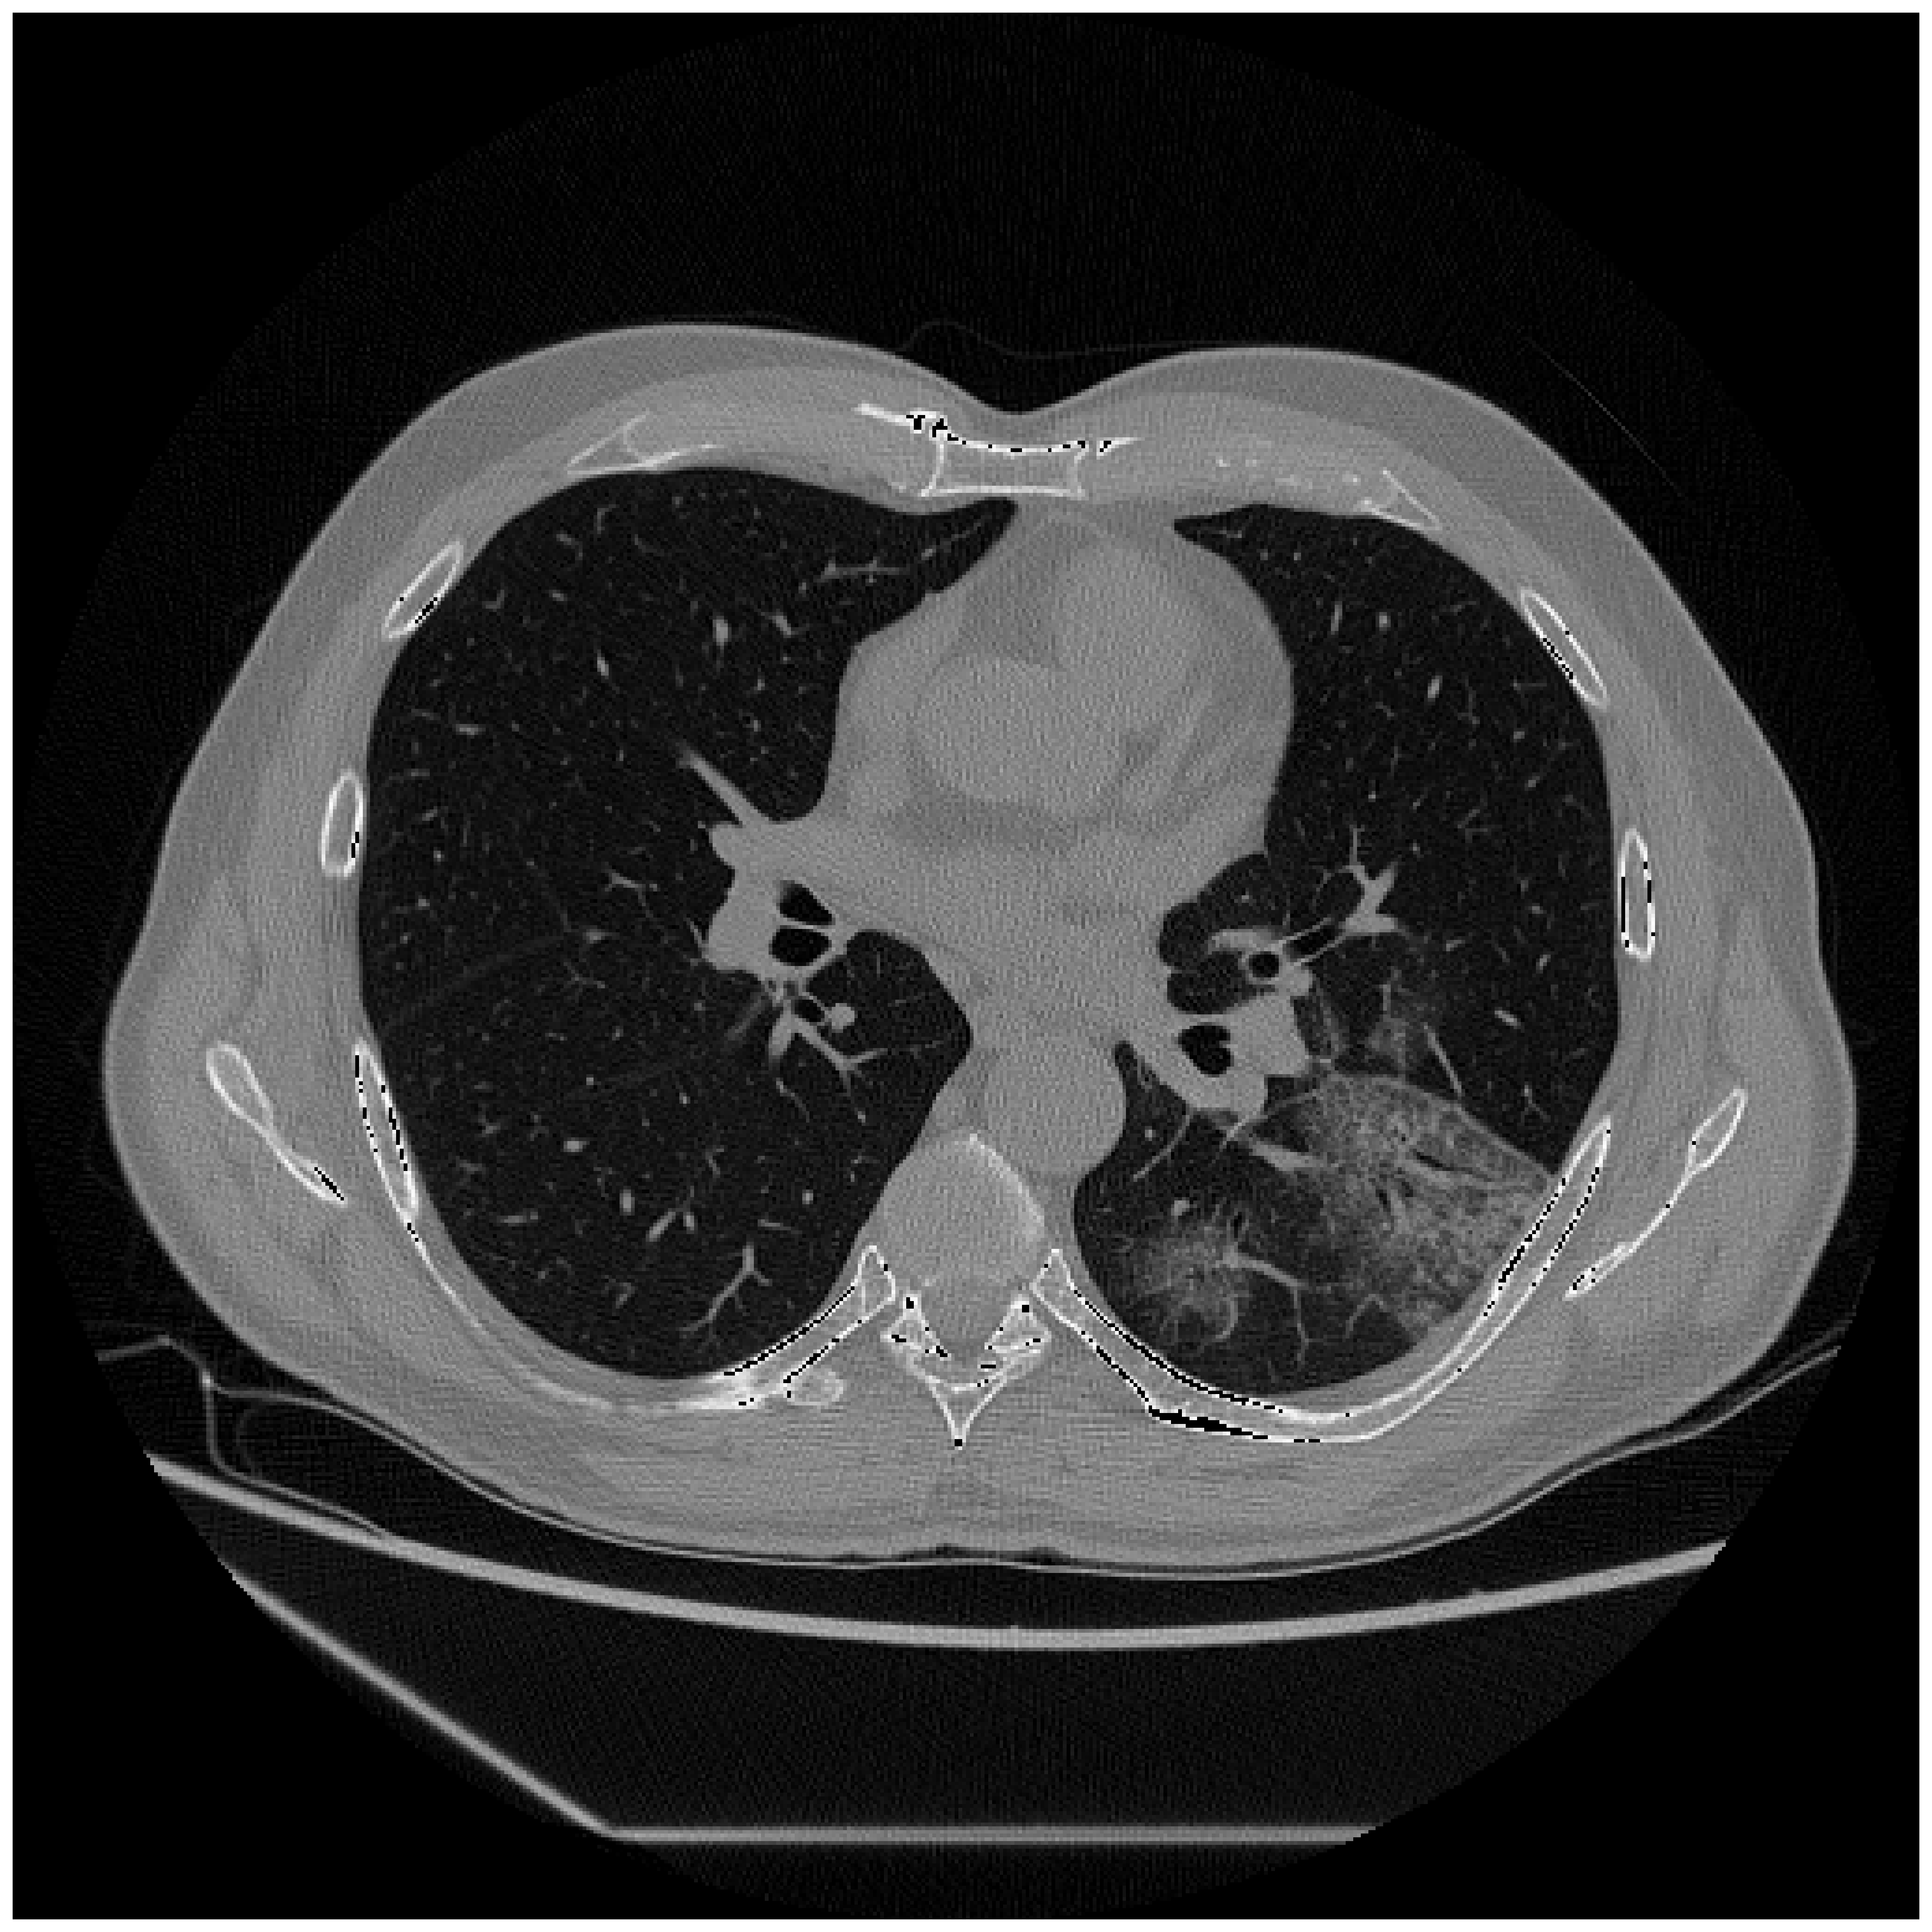
\includegraphics[scale=.12]{./img/GGO.png}			
		\end{column}
		\begin{column}{0.5\textwidth}
					\begin{block}{COVID-19}
					\begin{itemize}
						
						\item Viral(SARS-CoV-2) 
						
						\item Acute infectious disease
						
						\item Peculiar GGO and CS patterns
						
					\end{itemize}
				\end{block}			
				\begin{block}{Why Identify Them?}
					\begin{itemize}
						
						\item \textbf{To Help} diagnosis
						
						\item \textbf{To Monitor}:  
						\begin{itemize}
							\item the course of the disease
							
							\item the recovery of healed patients
						\end{itemize} 		
					\end{itemize}
				\end{block}				
		\end{column}
	\end{columns}	
	\end{frame}
\end{document}